\chapter{रक्त और परिसंचरण तंत्र}\label{ch:b2:blood-circulation}

1628 में विलियम हार्वे ने एक जोड़ लगाया। उनके आकलन से हृदय में लगभग दो
औंस \omterm{def:b2:blood-circulation:blood}{रक्त} समाता है और वह मिनट में सत्तर बार धड़कता है; और यदि हर धड़कन
पर उसका कोई अंश भी बाहर फेंका जाए, तो हृदय घंटे भर में पूरी देह के भार
से कई गुना पंप कर देगा। \omterm{def:b2:blood-circulation:blood}{रक्त} उस दर से बन और खप नहीं सकता, जैसा गैलेन ने
चौदह शताब्दियों तक पढ़ाया था; उसे घूम-घूमकर लौटना ही होगा। फिर उन्होंने
वह दिखा दिया: बाँह पर कोई डोरी बाँधिए, और उस डोरी के नीचे की \omterm{def:b2:blood-circulation:vessels}{शिराएँ}
फूलती हैं, ऊपर की नहीं; किसी \omterm{def:b2:blood-circulation:vessels}{शिरा} में \omterm{def:b2:blood-circulation:blood}{रक्त} को किसी कपाट के पार हाथ की
ओर दबाइए, और वह नहीं जाएगा। \omterm{def:b2:blood-circulation:blood}{रक्त} धमनियों से बाहर पंप किया जाता है,
\omterm{def:b2:blood-circulation:vessels}{शिराओं} से लौटता है, और पूरे पाँच लीटर हर मिनट हृदय से गुज़रते हैं। यह
अध्याय उसी बंद तंत्र के बारे में है --- कि \omterm{def:b2:blood-circulation:blood}{रक्त} है क्या, उसका मार्ग कैसे
तय होता है, महाधमनी से किसी \omterm{def:b2:blood-circulation:vessels}{केशिका} तक वाहिकाओं में उसके प्रवाह की
भौतिकी, और वह विनिमय, \omterm{def:b2:blood-circulation:vessels}{केशिकाओं} में, जो इस सबका मतलब है।

\section{रक्त}

\begin{definition}[रक्त की संरचना]\label{def:b2:blood-circulation:blood}
\index{रक्त}\index{प्लाज़्मा}\index{हीमैटोक्रिट}\index{लाल रक्त कोशिका}\index{बिंबाणु}
रक्त निलंबन में एक ऊतक है: किसी वयस्क में लगभग \qty{5}{L}, यानी
देह-द्रव्यमान का \qty{7}{\%}। अपकेंद्रित करने पर वह अलग होता है
\emph{प्लाज़्मा} में (\qty{55}{\%}: जल, \qty{70}{g/L} प्रोटीन ---
एल्ब्यूमिन, ग्लोब्युलिन, फ़ाइब्रिनोजन --- और वे लवण, शर्कराएँ, लिपिड,
गैसें तथा हॉर्मोन जो वह ढोता है) और कोशिकाओं में (\qty{45}{\%}, यानी
\emph{हीमैटोक्रिट}): \emph{लाल कोशिकाएँ} (प्रति लीटर $5\times 10^{12}$,
\qty{7}{\micro m} की उभयावतल बिना केंद्रक की चकतियाँ, हर एक में
\num{280} करोड़ हीमोग्लोबिन अणु ठुँसे, 120 दिन जीती और
मज्जा में दो लाख प्रति सेकंड बनतीं), \emph{श्वेत कोशिकाएँ}
(प्रति लीटर $7\times 10^{9}$: न्यूट्रोफ़िल, लसीकाणु, मोनोसाइट,
इओसिनोफ़िल, बेसोफ़िल, यानी प्रतिरक्षा की चलती भुजा), और
\emph{बिंबाणु} (प्रति लीटर $3\times 10^{11}$, मज्जा-कोशिकाओं के वे
टुकड़े जो घाव पाटते और स्कंदन शुरू करते हैं)। लाल कोशिकाएँ
ऑक्सीजन ढोती हैं --- पूर्ण संतृप्ति पर प्रति लीटर रक्त \qty{200}{mL},
यानी जल जितना घोलता है उससे सत्तर गुना --- और प्लाज़्मा बाक़ी सब कुछ,
जिसमें $\mathrm{CO_2}$ का वह \qty{20}{\%} भी है जो उन कोशिकाओं में
नहीं है, पेशियों की ऊष्मा त्वचा तक, और
\cref{ch:b2:cell-signalling} के हॉर्मोन अपने लक्ष्यों तक। रक्त
\emph{\omterm{thm:b2:blood-circulation:oncotic}{परासरणी दाब}} में एक विलयन भी है: उसके प्रोटीन,
जो \omterm{def:b2:blood-circulation:vessels}{केशिकाएँ} छोड़ नहीं सकते, लगभग \qty{25}{mmHg} की
परासरणी खिंचाई रखते हैं, और वही खिंचाई प्लाज़्मा को वाहिकाओं में बनाए
रखती है।
\end{definition}

\begin{omfigure}
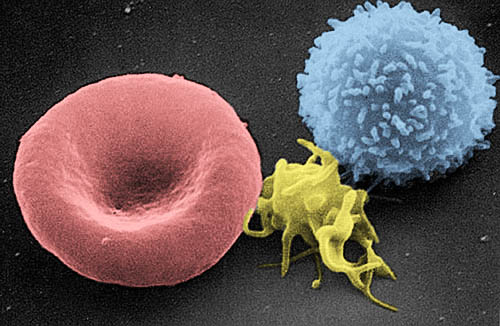
\includegraphics[width=0.5\linewidth]{images/book3/red-cells-nci.jpg}

{\small किसी क्रमवीक्षण इलेक्ट्रॉन सूक्ष्मदर्शी के नीचे एक लाल कोशिका,
एक \omterm{def:b2:blood-circulation:blood}{बिंबाणु} और एक श्वेत कोशिका (कोई लसीकाणु): \omterm{def:b2:blood-circulation:blood}{रक्त} के तीनों
कोशिकीय घटक, उसी पैमाने पर खींचे गए।}
\end{omfigure}

\begin{proposition}[रक्तस्तंभन]\label{prop:b2:blood-circulation:clotting}
\index{रक्तस्तंभन}\index{स्कंदन-सोपान}\index{फ़ाइब्रिन}
कटी हुई कोई वाहिका मिनटों के भीतर तीन चरणों में बंद कर दी जाती है। वह
वाहिका सिकुड़ती है; \omterm{def:b2:blood-circulation:blood}{बिंबाणु} खुले पड़े कोलैजन से चिपकते हैं, ऐसे
संकेत छोड़ते हैं जो और \omterm{def:b2:blood-circulation:blood}{बिंबाणु} बुलाते तथा सक्रिय करते हैं, और कोई डाट
बना देते हैं; और \omterm{def:b2:blood-circulation:blood}{प्लाज़्मा} प्रोटिएज़ों का कोई \emph{सोपान}, जिसमें हर एक
अगले को सक्रिय करता है (एक दर्जन स्कंदन कारक, जिनमें अधिकांश यकृत में
बनते हैं और कई को विटामिन K चाहिए), फ़ाइब्रिनोजन को अघुलनशील
\emph{फ़ाइब्रिन} में बदल देता है, जिसके तंतु उस डाट को बुनकर कोई थक्का
बना देते हैं। कोई सोपान प्रवर्धित करता है: उस प्रवर्तक का लेश
(क्षतिग्रस्त भित्ति से ऊतक कारक) ग्रामों भर फ़ाइब्रिन में अंत होता है।
उसे रोके रखना भी पड़ता है: \omterm{def:b2:blood-circulation:blood}{प्लाज़्मा} के प्रतिस्कंदक
(ऐंटीथ्रॉम्बिन, प्रोटीन C) और अक्षत अंतःस्तर पर वाले उस थक्के को उस घाव
तक सीमित रखते हैं, और दूसरा तंत्र, फ़ाइब्रिन-अपघटन, वाहिका के भरने के
साथ उसे घोल देता है। हीमोफ़ीलिया किसी एक कारक का अभाव है; कोई
घनास्रता वह थक्का है जहाँ कोई चाहा नहीं था, और धनी देशों में मृत्यु का
सबसे बड़ा कारण किसी हृद्- या मस्तिष्क-धमनी में कोई थक्का है।
\end{proposition}

\section{परिपथ}

\begin{definition}[खुला और बंद, एकल और दोहरा]\label{def:b2:blood-circulation:circuits}
\index{खुला परिसंचरण}\index{बंद परिसंचरण}\index{दोहरा परिसंचरण}\index{फुफ्फुसीय परिसंचरण}\index{दैहिक परिसंचरण}
किसी \emph{खुले} परिसंचरण में (कीट, अधिकांश मोलस्क) कोई हृदय
\omterm{def:b2:blood-circulation:blood}{रक्त} को किसी देह-गुहा में पंप करता है जहाँ वह अंगों को सीधे नहलाता है और
नीचे दाब पर लौटता है; प्रवाह धीमा तथा ख़राब निर्देशित है, और
कीटों ने गैस की समस्या \omterm{def:b2:blood-circulation:blood}{रक्त} से अलग कर ली है, वायु को
सीधे ऊतकों तक पहुँचाकर। किसी \emph{बंद} परिसंचरण में (वलयी,
शीर्षपाद, कशेरुकी) \omterm{def:b2:blood-circulation:blood}{रक्त} वाहिकाओं में ही रहता है और दाब पर
\omterm{def:b2:blood-circulation:vessels}{केशिकाओं} से होकर चलाया जाता है, ताकि उसका वितरण अंग-दर-अंग
नियंत्रित किया जा सके। मछलियों का परिपथ \emph{एकल} है: हृदय
$\to$ क्लोम $\to$ देह $\to$ हृदय, इसलिए \omterm{def:b2:blood-circulation:blood}{रक्त} ऊतकों तक उस
नीचे दाब पर पहुँचता है जो क्लोम-केशिकाओं के बाद बचा। स्तनियों और
पक्षियों का परिपथ \emph{दोहरा} है: दायाँ हृदय
\emph{फुफ्फुसीय} परिसंचरण चलाता है (फेफड़े, नीचा दाब, \qty{25}{mmHg}
प्रकुंचनी) और बायाँ हृदय, \omterm{def:b2:blood-circulation:blood}{रक्त} के लौट आने पर,
\emph{दैहिक} परिसंचरण (देह, ऊँचा दाब, \qty{120}{mmHg});
दोनों पंप श्रेणी में हैं और वही प्रवाह चलाते हैं, विश्राम में लगभग
मिनट भर में \qty{5}{L}। उभयचरों तथा अधिकांश सरीसृपों के हृदय में
एक ही निलय है जो दोनों धाराएँ कुछ-कुछ मिला देता है --- यानी वह
मध्यवर्ती अवस्था। दोहरा परिपथ ही किसी गर्म-रक्ती
उपापचय को संभव बनाता है: हर अंग तक ऊँचा दाब और उससे बचा हुआ
कोई फेफड़ा।
\end{definition}
\begin{proof}[प्रमाण-सामग्री]
हार्वे (1628) ने मात्रा से तर्क किया --- यानी ऊपर गिना गया वह निर्गम ---
और संरचना से: \omterm{def:b2:blood-circulation:vessels}{शिराओं} के वे कपाट, जिनका वर्णन फ़ैब्रिसियस ने
किया था, प्रवाह केवल हृदय की ओर आने देते हैं, जैसा उन्होंने किसी बँधी
बाँह की \omterm{def:b2:blood-circulation:vessels}{शिराओं} पर दबाकर दिखाया; हृदय के कपाट
प्रवाह केवल अलिंदों से निलयों में और निलयों से धमनियों में आने देते हैं;
और धमनियों में \omterm{def:b2:blood-circulation:blood}{रक्त} फुहार मारता है, \omterm{def:b2:blood-circulation:vessels}{शिराओं} में रिसता है। वे
\omterm{def:b2:blood-circulation:vessels}{केशिकाएँ} देख नहीं सके और उनका अनुमान लगाया; माल्पीगी ने उन्हें किसी मेंढक
के फेफड़े में 1661 में देखा, हार्वे की मृत्यु के चार वर्ष बाद।
\end{proof}

\begin{omfigure}
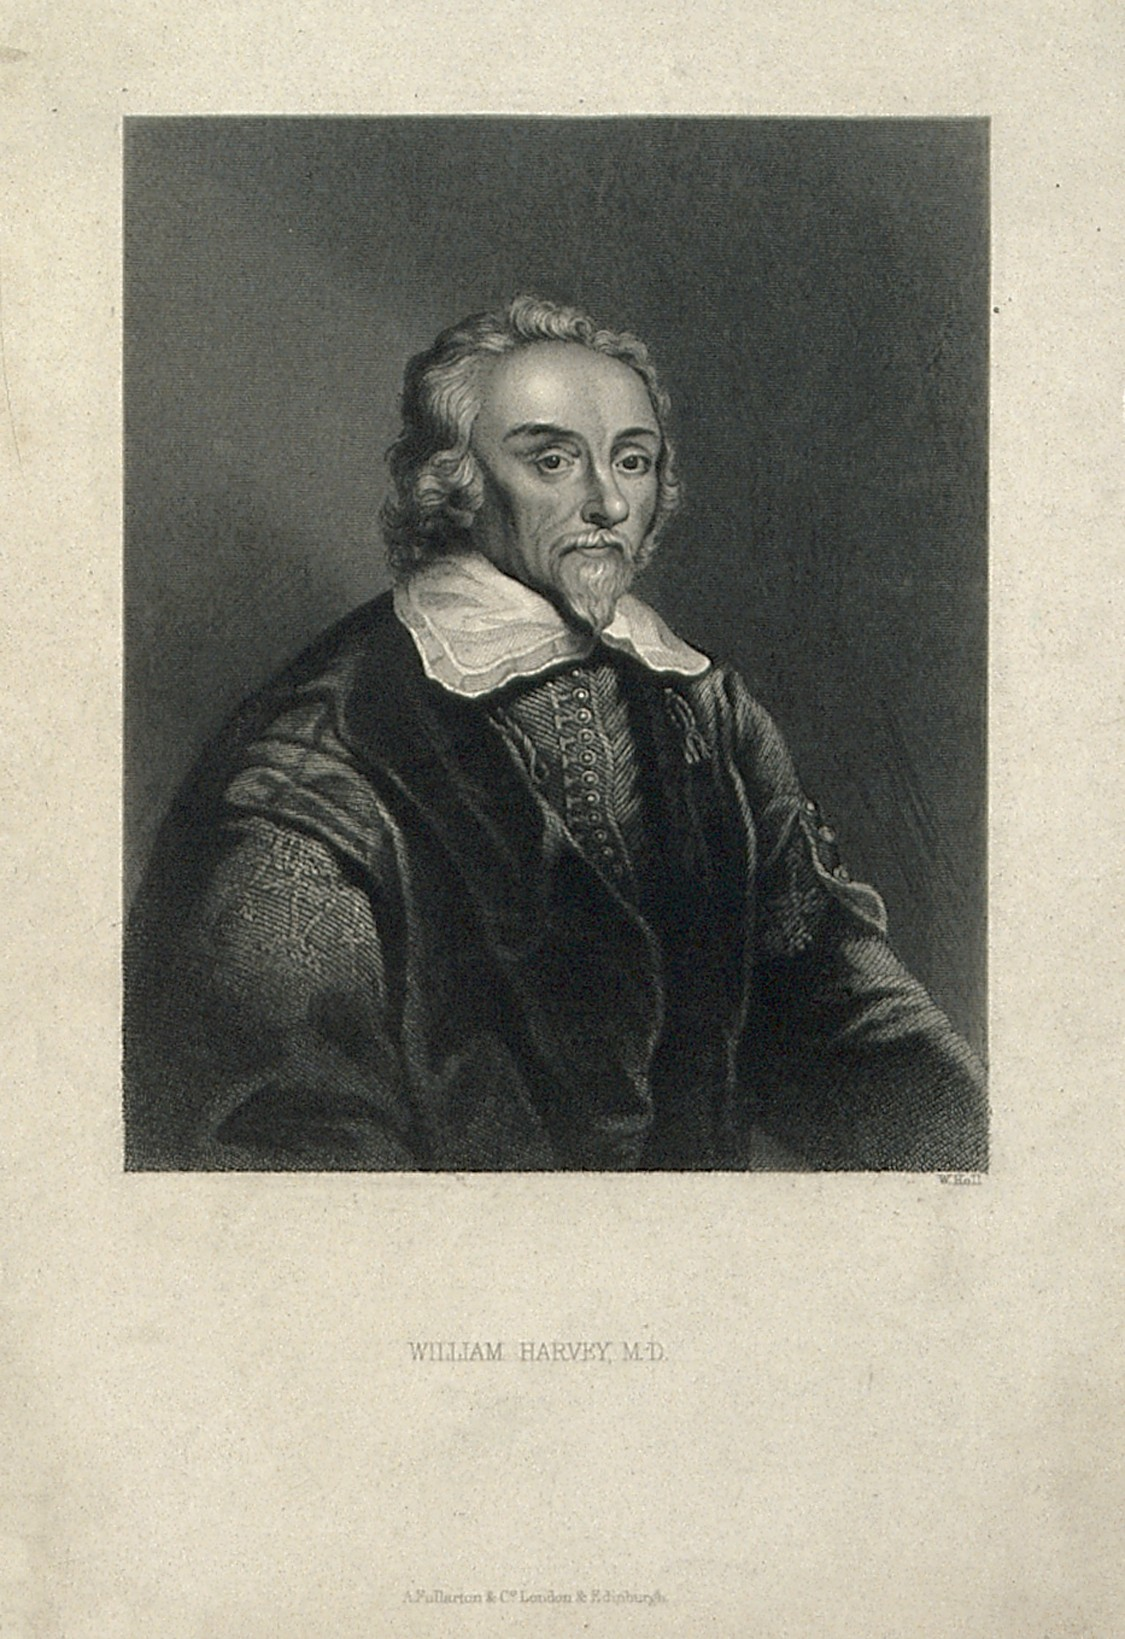
\includegraphics[width=0.3\linewidth]{images/book4/harvey.jpg}\hspace{0.05\linewidth}
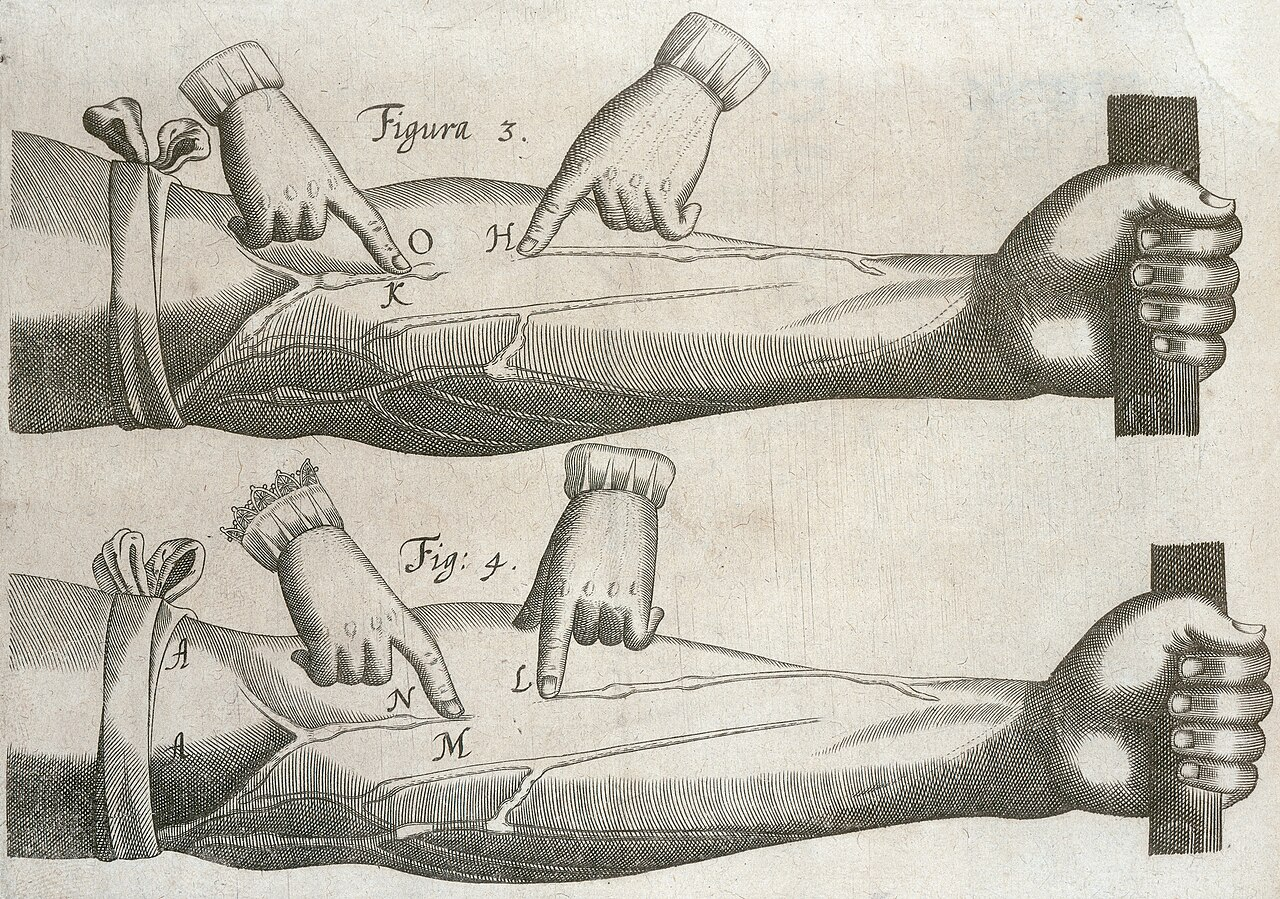
\includegraphics[width=0.42\linewidth]{images/book4/harvey-veins.jpg}

{\small विलियम हार्वे, और 1628 की उनकी पुस्तक का वह चित्रफलक: किसी
बँधी प्रबाहु की \omterm{def:b2:blood-circulation:vessels}{शिराएँ} उस डोरी के नीचे फूलती हैं, और हाथ की ओर
दबाया गया \omterm{def:b2:blood-circulation:blood}{रक्त} कपाटों पर रुक जाता है।}
\end{omfigure}

\begin{omfigure}
\begin{tikzpicture}[every node/.style={font=\scriptsize}, >=stealth]
  % lungs and body
  \node[draw, rounded corners, fill=omDef!12, minimum width=3.4cm, minimum height=0.9cm] (lung) at (0,3) {फेफड़े: फुफ्फुसीय केशिकाएँ};
  \node[draw, rounded corners, fill=omExo!25, minimum width=3.4cm, minimum height=0.9cm] (body) at (0,-3) {देह: दैहिक केशिकाएँ};
  % heart chambers
  \node[draw, fill=omDef!25, minimum width=1.3cm, minimum height=0.7cm] (ra) at (-1.6,0.6) {दायाँ अलिंद};
  \node[draw, fill=omDef!35, minimum width=1.3cm, minimum height=0.9cm] (rv) at (-1.6,-0.5) {दायाँ निलय};
  \node[draw, fill=omThm!20, minimum width=1.3cm, minimum height=0.7cm] (la) at (1.6,0.6) {बायाँ अलिंद};
  \node[draw, fill=omThm!35, minimum width=1.3cm, minimum height=0.9cm] (lv) at (1.6,-0.5) {बायाँ निलय};
  \draw[->, thick] (ra) -- (rv); \draw[->, thick] (la) -- (lv);
  % pulmonary circuit
  \draw[->, very thick, omDef] (rv.west) -- ++(-1.4,0) |- (lung.west) node[pos=0.25, left, align=right] {फुफ्फुस धमनी\\\qty{25}{mmHg}};
  \draw[->, very thick, omThm] (lung.east) -| (la.east) node[pos=0.75, right, align=left] {फुफ्फुस शिराएँ\\ऑक्सीजनित};
  % systemic circuit
  \draw[->, very thick, omThm] (lv.east) -- ++(1.4,0) |- (body.east) node[pos=0.25, right, align=left] {महाधमनी\\\qty{120}{mmHg}};
  \draw[->, very thick, omDef] (body.west) -| (ra.west);
  \node[omDef, anchor=east, align=right] at (-2.45,-1.6) {महाशिराएँ\\\qty{5}{mmHg}};
  \node[anchor=north, align=center] at (0,-3.7) {दोनों परिपथों से वही प्रवाह:\\विश्राम में \qty{5}{L/min}};
\end{tikzpicture}

{\small \omterm{def:b2:blood-circulation:circuits}{दोहरा परिसंचरण}। दायाँ हृदय \omterm{def:b2:blood-circulation:blood}{रक्त} को
नीचे दाब पर फेफड़ों से भेजता है; बायाँ हृदय उसे ऊँचे दाब पर देह भर
घुमाता है; और दोनों पंप, श्रेणी में, प्रति मिनट वही आयतन
चलाते हैं।}
\end{omfigure}

\section{वाहिकाएँ और प्रवाह की भौतिकी}

\begin{definition}[वाहिका-वृक्ष]\label{def:b2:blood-circulation:vessels}
\index{धमनी}\index{धमनिका}\index{केशिका}\index{शिरा}
\omterm{def:b2:blood-circulation:blood}{रक्त} हृदय से \emph{धमनियों} से होकर निकलता है: मोटी भित्ति वाली ऐसी
नलियाँ जिनकी प्रत्यास्थ परतें हर धड़कन पर खिंचती और धड़कनों के बीच
सिकुड़ती हैं, और स्पंदों को किसी स्थिरतर प्रवाह में चिकना कर देती हैं
(महाधमनी \qty{2.5}{cm} चौड़ी है)। वे \emph{धमनिकाओं} में शाखित होती हैं,
यानी मिलीमीटर के दसवें भाग या उससे छोटी ऐसी वाहिकाएँ जिनकी भित्तियाँ
अधिकतर चिकनी पेशी हैं: सिकुड़कर या ढीली होकर कोई धमनिका अपनी त्रिज्या
बदलती है और, इस तरह, अपना प्रतिरोध बहुत ज़ोर से --- धमनिकाएँ इस
परिसंचरण की टोंटियाँ हैं और अधिकांश दाब-पात की जगह। ये
\emph{केशिकाओं} में खुलती हैं: यानी \qtyrange{5}{10}{\micro m} की गुहा
के चारों ओर लिपटी एकल अंतःस्तरी कोशिका की नलियाँ, लगभग
\qty{1}{mm} लंबी, जिनमें से कोई चालीस अरब हैं और जिनका कुल पृष्ठ
\qty{600}{m^2} के पास है, और जिनकी भित्तियों के आरपार सारा विनिमय होता है।
केशिकाएँ शिरिकाओं और \emph{शिराओं} में बहती हैं: पतली भित्ति वाली,
फैलनशील, नीचे दाब पर \omterm{def:b2:blood-circulation:blood}{रक्त} का दो तिहाई थामे हुए, और ऐसे
कपाटों वाली जो पेशियों के दबाने के साथ प्रवाह हृदय की ओर रखते हैं।
हर वाहिका \emph{अंतःस्तर} की एक ही परत से भीतर से मढ़ी है, जो कोई
निष्क्रिय अस्तर नहीं बल्कि एक ग्रंथि है ---
वह धमनिका को ढीला करने के लिए नाइट्रिक ऑक्साइड छोड़ती है, और ऐसे संकेत
जो श्वेत कोशिकाएँ बुलाते हैं --- और एक छन्ना।
\end{definition}

\begin{omfigure}
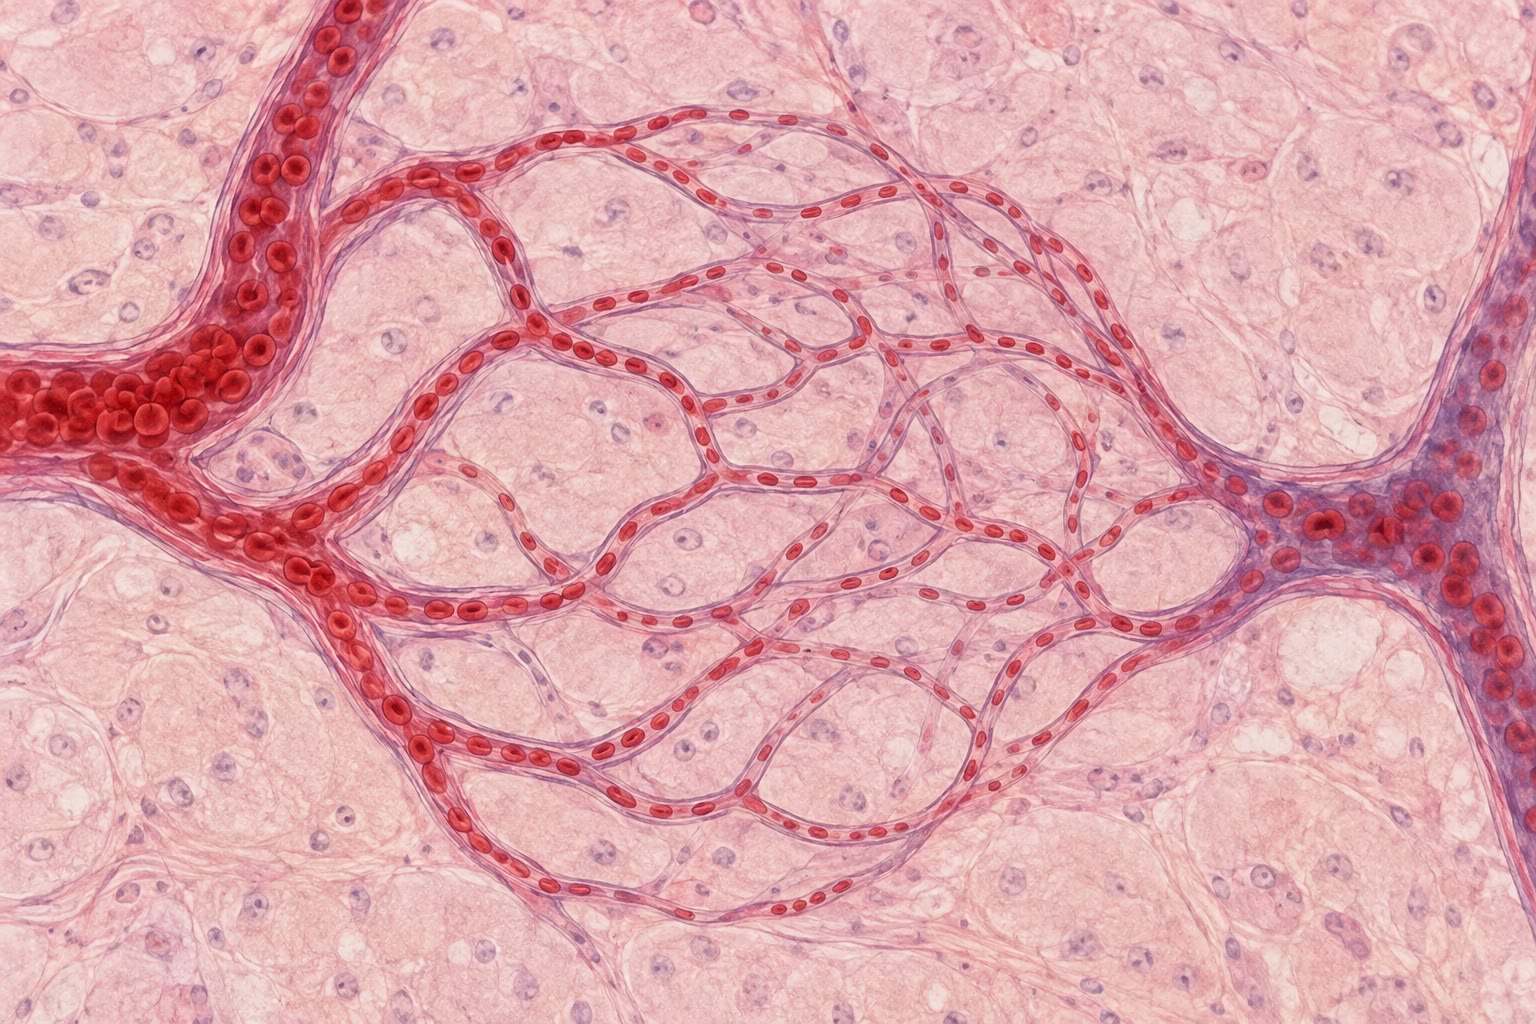
\includegraphics[width=0.55\linewidth]{images/book4/ai/b4-16-capillary-bed.jpg}

{\small कोई केशिका-शय्या: कोई \omterm{def:b2:blood-circulation:vessels}{धमनिका} \omterm{def:b2:blood-circulation:vessels}{केशिकाओं} के किसी जाल को
पोसती हुई, जिनमें लाल कोशिकाएँ एक-एक कर चलती हैं, और किसी शिरिका में फिर मिलती हुई।}
\end{omfigure}

\begin{theorem}[प्वाज़ेई का नियम और वाहिकीय प्रतिरोध]\label{thm:b2:blood-circulation:poiseuille}
\index{प्वाज़ेई का नियम}\index{वाहिकीय प्रतिरोध}
स्थिर प्रवाह $Q$, जो $\eta$ श्यानता के किसी तरल का $r$ त्रिज्या तथा
$L$ लंबाई की किसी नली से होकर $\Delta P$ दाबांतर के अधीन है, यह
है:
\[
Q = \frac{\pi r^{4}}{8\eta L}\,\Delta P, \qquad \text{इसलिए}\qquad
R \equiv \frac{\Delta P}{Q} = \frac{8\eta L}{\pi r^{4}} .
\]
प्रतिरोध त्रिज्या की \emph{चौथी घात} से गिरता है: कोई
\omterm{def:b2:blood-circulation:vessels}{धमनिका} जो अपनी त्रिज्या \qty{20}{\%} घटा ले वह अपना
प्रतिरोध $1/0.8^{4} = 2.4$ से गुणा कर लेती है, और जो उसे आधा कर ले वह 16 से। इसी से
धमनिका-पेशी के कुछ मिलीमीटर पूरी देह का \omterm{def:b2:blood-circulation:blood}{रक्त} फिर से भेज
सकते हैं --- भोजन के बाद आँत को, व्यायाम में पेशियों को, गर्मी में
त्वचा को --- और इसी से दाब छोटी धमनियों के
\qty{95}{mmHg} से गिरकर \omterm{def:b2:blood-circulation:vessels}{केशिकाओं} के प्रवेश पर
\qty{35}{mmHg} रह जाता है, और वह भी लगभग पूरा
\omterm{def:b2:blood-circulation:vessels}{धमनिकाओं} के आरपार, जबकि महाधमनी के साथ वाला पात पारे के मिलीमीटर के
किसी अंश भर है।
\end{theorem}
\begin{proof}
स्थिर धारारेखी प्रवाह में वह तरल संकेंद्री खोलों में चलता है; खोलों
के बीच का श्यान बल उस दाब को संतुलित करता है। $s < r$ त्रिज्या के
बेलन के लिए दाब-बल $\pi s^{2}\Delta P$
उसके पृष्ठ पर के श्यान कर्षण $2\pi s L\,\eta\,(-\mathrm{d}v/
\mathrm{d}s)$ के बराबर है, इसलिए $\mathrm{d}v/\mathrm{d}s = -s\Delta P/(2\eta L)$
और, $v(r) = 0$ के साथ, $v(s) = (\Delta P/4\eta L)(r^{2} - s^{2})$ --- यानी कोई
परवलयी परिच्छेदिका। उस वेग को अनुप्रस्थ काट पर समाकलित करने से,
$Q = \int_{0}^{r} v\,2\pi s\,\mathrm{d}s = (\pi\Delta P/2\eta L)
\int_{0}^{r}(r^{2}s - s^{3})\,\mathrm{d}s = \pi r^{4}\Delta P/8\eta
L$। (\omterm{def:b2:blood-circulation:blood}{रक्त} पूरी तरह कोई सरल तरल नहीं है और धमनियाँ दृढ़ नहीं हैं,
पर वह चौथी-घात नियम किसी देह चलाने भर को ठीक टिकता है।)
\end{proof}

\begin{theorem}[संतति: रक्त कहाँ धीमा पड़ता है]\label{thm:b2:blood-circulation:continuity}
\index{संतति समीकरण}
वही आयतन प्रति सेकंड उस वृक्ष के हर स्तर से गुज़रता है, इसलिए किसी
स्तर पर माध्य वेग $v = Q/A$ है, जिसमें $A$ उस स्तर की सारी वाहिकाओं की
\emph{कुल} अनुप्रस्थ काट है। महाधमनी
(\qty{3}{cm^2}) \qty{5}{L/min} को \qty{28}{cm/s} पर ढोती है; जबकि
\omterm{def:b2:blood-circulation:vessels}{केशिकाएँ}, जिनकी कुल काट \qty{3000}{cm^2} के पास है, उसे
\qty{0.03}{cm/s} पर, इसलिए कोई लाल कोशिका किसी \omterm{def:b2:blood-circulation:vessels}{केशिका} को पार करने में
कोई तीन सेकंड लेती है --- यानी उसकी ऑक्सीजन के बाहर विसरित होने भर का समय
(\cref{ch:b2:unicellular-diversity}: कोई माइक्रोमीटर किसी
मिलीसेकंड में)। \omterm{def:b2:blood-circulation:vessels}{शिराएँ}, जिनकी कुल काट \omterm{def:b2:blood-circulation:vessels}{केशिकाओं} से छोटी है,
\omterm{def:b2:blood-circulation:blood}{रक्त} को महाशिराओं में फिर \qty{10}{cm/s} तक तेज़ कर देती हैं। वह
वृक्ष ऐसे बना है कि \omterm{def:b2:blood-circulation:blood}{रक्त} ठीक वहीं धीमा हो जहाँ उसे
विनिमय करना है, और बाक़ी हर जगह तेज़।
\end{theorem}
\begin{proof}
आयतन का संरक्षण: जो किसी स्तर में प्रति सेकंड घुसता है वही निकलता है,
इसलिए $Q = A\,v$ हर स्तर पर वही है। $\qty{5}{L/min} =
\qty{83}{cm^3/s}$; $83/3 = \qty{28}{cm/s}$; $83/3000 =
\qty{0.028}{cm/s}$।
\end{proof}

\begin{omfigure}
\begin{tikzpicture}
\begin{axis}[
  width=0.9\linewidth, height=6.4cm,
  axis x line=bottom, axis y line=left,
  xmin=0, xmax=7, ymin=0, ymax=130,
  xtick={0.5,1.5,2.5,3.5,4.5,5.5,6.5},
  xticklabels={महाधमनी, धमनियाँ, धमनिकाएँ, केशिकाएँ, शिरिकाएँ, शिराएँ, महाशिराएँ},
  x tick label style={font=\scriptsize, rotate=30, anchor=north east},
  ylabel={दाब (\unit{mmHg})}, ylabel style={font=\small, omThm},
  tick label style={font=\small}, ytick={0,40,80,120},
  legend style={font=\scriptsize, at={(0.97,0.95)}, anchor=north east, draw=none},
  clip=false,
]
\addplot[very thick, omThm] coordinates {(0,120) (0.5,118) (1,110) (1.5,100) (2,95) (2.5,60) (3,35) (3.5,25) (4,15) (4.5,12) (5,8) (5.5,5) (6,4) (6.5,3) (7,2)};
\addlegendentry{माध्य दाब}
\addplot[very thick, omThm, dashed] coordinates {(0,120) (0.5,120) (1,125) (1.5,120) (2,100)};
\addplot[very thick, omThm, dashed] coordinates {(0,80) (0.5,80) (1,80) (1.5,82) (2,88)};
\addlegendentry{प्रकुंचनी और अनुशिथिलनी}
\end{axis}
\begin{axis}[
  width=0.9\linewidth, height=6.4cm,
  axis x line=none, axis y line=right,
  xmin=0, xmax=7, ymin=0, ymax=32,
  ylabel={वेग (\unit{cm/s})}, ylabel style={font=\small, omDef},
  tick label style={font=\small}, ytick={0,10,20,30},
  legend style={font=\scriptsize, at={(0.97,0.72)}, anchor=north east, draw=none},
  clip=false,
]
\addplot[very thick, omDef] coordinates {(0,28) (0.5,26) (1,18) (1.5,10) (2,5) (2.5,1.5) (3,0.3) (3.5,0.03) (4,0.3) (4.5,1.5) (5,4) (5.5,7) (6,9) (6.5,10) (7,10)};
\addlegendentry{माध्य वेग}
\end{axis}
\end{tikzpicture}

{\small \omterm{def:b2:blood-circulation:circuits}{दैहिक परिसंचरण} के साथ दाब (लाल) और माध्य वेग
(नीला)। स्पंद धमनियों में चिकना कर दिया जाता है, दाब
अधिकतर \omterm{def:b2:blood-circulation:vessels}{धमनिकाओं} के आरपार गिरता है, और \omterm{def:b2:blood-circulation:blood}{रक्त}
\omterm{def:b2:blood-circulation:vessels}{केशिकाओं} में सबसे धीमा है, जहाँ कुल अनुप्रस्थ काट महाधमनी से
हज़ार गुना है।}
\end{omfigure}

\begin{theorem}[प्रत्यास्थ धमनी एक जलाशय के रूप में]\label{thm:b2:blood-circulation:windkessel}
\index{विंडकेसल}\index{अनुपालिता!धमनीय}\index{स्पंद दाब}
हृदय झोंकों में निकालता है; ऊतकों को लगभग स्थिर
प्रवाह मिलता है। वह चिकनापन बड़ी धमनियाँ लाती हैं: वे निष्कासन के
दौरान खिंचती हैं, आघात-आयतन का कुछ भाग संचित करती हैं, और
अनुशिथिलन में सिकुड़कर उसे आगे चला देती हैं। यदि उन धमनियों की कोई
\emph{अनुपालिता} $C$ हो (प्रति इकाई दाब संचित आयतन) और \omterm{def:b2:blood-circulation:vessels}{धमनिकाओं} का कोई
प्रतिरोध $R$, तो अनुशिथिलन के दौरान, महाधमनी-कपाट बंद रहते,
दाब इस तरह क्षीण होता है:
\[
P(t) = P_{s}\,e^{-t/RC},
\]
इसलिए $t_d$ अवधि के किसी अनुशिथिलन के बाद अनुशिथिलनी दाब
$P_s e^{-t_d/RC}$ है: $R = \qty{1}{mmHg.s/mL}$, $C =
\qty{2}{mL/mmHg}$ और $t_d = \qty{0.8}{s}$ के साथ, कोई प्रकुंचनी
\qty{120}{mmHg} गिरकर \qty{80}{mmHg} रह जाता है। कोई कड़ी महाधमनी (छोटा
$C$, जैसा बुढ़ापे में) दाब को धड़कनों के बीच और नीचे गिरने
और निष्कासन के दौरान और ऊपर चढ़ने देती है: \emph{\omterm{thm:b2:blood-circulation:windkessel}{स्पंद दाब}} चौड़ा हो जाता है,
और हृदय किसी ऊँचे शिखर के विरुद्ध काम करता है।
\end{theorem}
\begin{proof}
अनुशिथिलन के दौरान धमनियों में \omterm{def:b2:blood-circulation:blood}{रक्त} घुसता नहीं और \omterm{def:b2:blood-circulation:blood}{रक्त} उनसे
\omterm{def:b2:blood-circulation:vessels}{धमनिकाओं} से होकर $Q = P/R$ पर निकलता है; धमनीय आयतन
$\mathrm{d}V/\mathrm{d}t = -P/R$ से गिरता है, और चूँकि $\mathrm{d}V = C\,
\mathrm{d}P$, इसलिए $C\,\mathrm{d}P/\mathrm{d}t = -P/R$, जिसका हल है
$RC$ काल-नियतांक वाला वह चरघातांकी। $RC = \qty{2}{s}$ के साथ:
$120\,e^{-0.4} = \qty{80}{mmHg}$।
\end{proof}

\section{केशिकाओं में विनिमय}

\begin{proposition}[विनिमय के दो प्रकार]\label{prop:b2:blood-circulation:exchange}
\index{केशिका विनिमय}\index{स्टार्लिंग बल}\index{शोफ}\index{लसीका}
केशिका-भित्ति के आरपार विलेय \emph{विसरण} से चलते हैं --- गैसें
और लिपिड कोशिकाओं से होकर, जल तथा छोटे विलेय उनके बीच की
दरारों से होकर, उस विशाल क्षेत्रफल और उस छोटी दूरी पर जो उस अभिवाह को
प्रचुर बना देते हैं (फ़िक का नियम, जैसा
\cref{ch:b2:mammal-reproduction} की जरायु के लिए) --- और जल
\emph{स्थूल प्रवाह} से चलता है, जो दो दाबों के संतुलन से चलाया जाता है।
\omterm{def:b2:blood-circulation:vessels}{केशिका} में द्रवस्थैतिक दाब, $P_c$, तरल को बाहर धकेलता है; और
\omterm{def:b2:blood-circulation:blood}{प्लाज़्मा} प्रोटीनों का \omterm{thm:b2:blood-circulation:oncotic}{परासरणी दाब}, $\pi_c$, उसे भीतर खींचता है
(\emph{\omterm{prop:b2:blood-circulation:exchange}{स्टार्लिंग बल}})। धमनीय सिरे पर $P_c \approx
\qty{35}{mmHg}$ $\pi_c \approx \qty{25}{mmHg}$ से बड़ा है और तरल
छनकर निकलता है; शिरीय सिरे पर $P_c \approx \qty{15}{mmHg}$ है और तरल
फिर सोख लिया जाता है; पूरी देह पर प्रतिदिन लगभग \qty{20}{L} छनकर
निकलते हैं और \qty{17}{L} लौटते हैं, और \qty{3}{L} का वह शेष, उन
प्रोटीनों समेत जो रिस गए, \emph{लसीका} वाहिकाएँ इकट्ठा करती हैं
और गले पर \omterm{def:b2:blood-circulation:vessels}{शिराओं} में लौटा देती हैं। \emph{शोफ} --- यानी ऊतकों में
तरल से सूजन --- तब आता है जब वह संतुलन डगमगाए:
ऊँचा शिरीय दाब (हृद्-विफलता), नीचा \omterm{def:b2:blood-circulation:blood}{प्लाज़्मा} प्रोटीन
(भुखमरी, यकृत या वृक्क का रोग), रिसती \omterm{def:b2:blood-circulation:vessels}{केशिकाएँ}
(शोथ), या अवरुद्ध लसीका वाहिकाएँ।
\end{proposition}

\begin{omfigure}
\begin{tikzpicture}[every node/.style={font=\scriptsize}, >=stealth]
  % capillary
  \draw[thick, fill=omThm!10] (0,0) rectangle (9,1.2);
  \node[left] at (-0.1,0.6) {धमनिका};
  \node[right] at (9.1,0.6) {शिरिका};
  \draw[->, very thick, omThm] (0.3,0.6) -- (8.7,0.6);
  % pressures
  \node[above, align=center] at (1.5,1.3) {धमनीय सिरा\\$P_c = 35$, $\pi_c = 25$};
  \node[above, align=center] at (7.5,1.3) {शिरीय सिरा\\$P_c = 15$, $\pi_c = 25$};
  \foreach \x in {0.8,1.5,2.2} \draw[->, thick, omDef] (\x,0) -- (\x,-0.7);
  \node[below, align=center, omDef] at (1.5,-0.75) {शुद्ध $+10$ mmHg:\\छनन};
  \foreach \x in {6.8,7.5,8.2} \draw[->, thick, omDef] (\x,-0.7) -- (\x,0);
  \node[below, align=center, omDef] at (7.5,-0.75) {शुद्ध $-10$ mmHg:\\पुनरवशोषण};
  \draw[->, thick, omExo!70!black] (4.5,-0.4) -- (4.5,-1.6) node[below, align=center] {अतिरेक लसीका को:\\प्रतिदिन \qty{3}{L}};
  \node[align=center] at (4.5,-0.15) {अंतरालीय तरल};
\end{tikzpicture}

{\small किसी \omterm{def:b2:blood-circulation:vessels}{केशिका} के साथ \omterm{prop:b2:blood-circulation:exchange}{स्टार्लिंग बल}। द्रवस्थैतिक दाब
तरल को बाहर धकेलता है और \omterm{def:b2:blood-circulation:blood}{प्लाज़्मा} प्रोटीनों का \omterm{thm:b2:blood-circulation:oncotic}{परासरणी दाब} उसे
वापस खींचता है; धमनीय सिरे पर छनन शिरीय सिरे के पुनरवशोषण से
बड़ा है, और लसीका वह अंतर लौटा देती है।}
\end{omfigure}

\begin{theorem}[परासरणी दाब]\label{thm:b2:blood-circulation:oncotic}
\index{परासरणी दाब}\index{एल्ब्यूमिन}
किसी ऐसे विलेय के $c$ मोल प्रति लीटर का विलयन जो किसी झिल्ली को पार
नहीं कर सकता उसके आरपार परासरण दाब $\pi = cRT$ डालता है (वान्ट
हॉफ़)। \omterm{def:b2:blood-circulation:blood}{प्लाज़्मा} एल्ब्यूमिन, यानी \qty{66}{kg/mol} मोलर द्रव्यमान के किसी
प्रोटीन का \qty{40}{g/L}, $c = \qty{0.6}{mmol/L}$ है और $\pi =
0.6\times 8.314\times 310 = \qty{1.55}{kPa} \approx \qty{12}{mmHg}$ देता है;
और बाक़ी प्रोटीन तथा वे अतिरिक्त आयन जिन्हें एल्ब्यूमिन का ऋण
आवेश रोके रखता है, कुल को लगभग \qty{25}{mmHg} तक ले आते हैं।
\omterm{def:b2:blood-circulation:blood}{प्लाज़्मा} का सोडियम क्लोराइड, \qty{150}{mmol/L} पर,
\qty{5800}{mmHg} डालता --- पर वह केशिका-भित्ति स्वतंत्र रूप से पार कर
जाता है और उसके आरपार कुछ नहीं डालता। उस \omterm{def:b2:blood-circulation:vessels}{केशिका} के लिए जो मायने रखता है वह है
प्रोटीन: एल्ब्यूमिन आधा कीजिए, जैसे उस वृक्क-रोग में जो उसे
मूत्र में खो देता है, और वह सोखती खिंचाई आधी हो जाती है, तरल
ऊतकों में जमा होता है, और वह रोगी सूज जाता है।
\end{theorem}
\begin{proof}
$\qty{40}{g/L}/\qty{66000}{g/mol} = \qty{6.1e-4}{mol/L} =
\qty{0.61}{mol/m^3}$; $\pi = cRT = 0.61\times 8.314\times 310 =
\qty{1570}{Pa}$; $\qty{1}{mmHg} = \qty{133}{Pa}$, इसलिए \qty{11.8}{mmHg}।
वान्ट हॉफ़ का नियम स्वयं वह तनु-विलयन सीमा है जो
वर्ष 1 के खंड में निकाली गई थी।
\end{proof}

\begin{example}[किसी परिवहन तंत्र के रूप में परिसंचरण]\label{ex:b2:blood-circulation:transport}
केशिका-भित्ति के \qty{600}{m^2} से होकर मिनट भर में पाँच लीटर कोई
अद्वितीय वितरण-सेवा है। वह हर कोशिका तक ऑक्सीजन
कुछ ही कोशिका-व्यासों के भीतर लाती है (देह की कोई कोशिका किसी \omterm{def:b2:blood-circulation:vessels}{केशिका}
से \qty{20}{\micro m} से दूर नहीं है), उसकी $\mathrm{CO_2}$,
लैक्टेट तथा यूरिया हटाती है, यकृत की ग्लूकोज़ मस्तिष्क तक और
वसा-भंडारों के वसीय अम्ल पेशियों तक ढोती है,
\cref{ch:b2:cell-signalling} के हॉर्मोन एक ग्रंथि से देह के हर
ग्राही तक मिनट भर में बाँटती है, केंद्र की ऊष्मा
त्वचा तक और वापस चलाती है, और श्वेत कोशिकाएँ किसी घाव तक घंटों के भीतर
पहुँचा देती है। वही उसकी भेद्यता भी है: कोई थक्का, कोई रक्तस्राव या कोई
चूकता पंप यह सब एक साथ रोक देता है, और मस्तिष्क, जो कोई ईंधन
संचित नहीं रखता, सेकंडों में चूक जाता है। पुस्तक के इस भाग का शेष उस
पंप के बारे में है (\cref{ch:b2:heart}) और इस बारे में कि दाब कैसे
नियंत्रित होता है ताकि खड़े होने, दौड़ने और \omterm{def:b2:blood-circulation:blood}{रक्त} बहने के बीच वह सेवा
चलती रहे (\cref{ch:b2:blood-pressure})।
\end{example}

\section{अभ्यास}

\begin{exercise}[$\star$]\label{exo:b2:blood-circulation:1}
\omterm{def:b2:blood-circulation:blood}{रक्त} की आयतन के हिसाब से संरचना, और हर कोशिकीय घटक की संख्या,
आकार तथा कार्य बताइए।
\end{exercise}

\begin{exercise}[$\star$]\label{exo:b2:blood-circulation:2}
किसी मछली और किसी स्तनी का परिपथ खींचिए, दाब अंकित कीजिए, और
कहिए कि दोहरा परिपथ क्या पाता है।
\end{exercise}

\begin{exercise}[$\star$]\label{exo:b2:blood-circulation:3}
हर वाहिका-प्रकार के लिए --- \omterm{def:b2:blood-circulation:vessels}{धमनी}, \omterm{def:b2:blood-circulation:vessels}{धमनिका}, \omterm{def:b2:blood-circulation:vessels}{केशिका}, \omterm{def:b2:blood-circulation:vessels}{शिरा} --- उसकी
भित्ति-संरचना और जिस कार्य में वह लगती है, बताइए।
\end{exercise}

\begin{exercise}[$\star$]\label{exo:b2:blood-circulation:4}
हार्वे का मात्रा वाला तर्क आधुनिक अंकों से फिर खड़ा कीजिए:
प्रति धड़कन \qty{70}{mL}, मिनट भर में \num{72} धड़कनें, \qty{5}{L} \omterm{def:b2:blood-circulation:blood}{रक्त}।
\end{exercise}

\begin{exercise}[$\star\star$]\label{exo:b2:blood-circulation:5}
\qty{5}{L/min} ढोती महाधमनी (त्रिज्या \qty{1.25}{cm},
लंबाई \qty{40}{cm}, $\eta = \qty{3e-3}{Pa.s}$) के साथ वाला दाब-पात
प्वाज़ेई के नियम से पास्कलों में तथा mmHg में निकालिए। टिप्पणी कीजिए।
\end{exercise}

\begin{exercise}[$\star\star$]\label{exo:b2:blood-circulation:6}
\qty{15}{\micro m} त्रिज्या की कोई \omterm{def:b2:blood-circulation:vessels}{धमनिका} सिकुड़कर
\qty{12}{\micro m} की हो जाती है, फिर फैलकर \qty{20}{\micro m} की। हर
स्थिति में उसका प्रतिरोध किस गुणक से बदलता है, और अचल दाब पर उसका
प्रवाह?
\end{exercise}

\begin{exercise}[$\star\star$]\label{exo:b2:blood-circulation:7}
महाधमनी की अनुप्रस्थ काट \qty{3}{cm^2} है और \omterm{def:b2:blood-circulation:vessels}{केशिकाओं} की कुल
\qty{3000}{cm^2}; प्रवाह \qty{5}{L/min} है। हर एक में माध्य
वेग, और किसी \qty{1}{mm} \omterm{def:b2:blood-circulation:vessels}{केशिका} में किसी लाल कोशिका का बिताया
काल निकालिए। व्यायाम के दौरान निर्गम चढ़कर
\qty{25}{L/min} हो जाता है और पेशी-केशिकाएँ खुल जाती हैं: उस
पारगमन-काल का क्या होता है?
\end{exercise}

\begin{exercise}[$\star\star$]\label{exo:b2:blood-circulation:8}
दोनों सिरों पर $P_c = 35$ तथा \qty{15}{mmHg}, $\pi_c =
\qty{25}{mmHg}$, और अंतरालीय दाब नगण्य होने पर, हर सिरे पर शुद्ध
छनन दाब निकालिए। यदि शिरीय दाब इतना चढ़ जाए कि शिरीय सिरे पर
$P_c$ \qty{28}{mmHg} हो जाए, तो क्या होता है?
\end{exercise}

\begin{exercise}[$\star\star$]\label{exo:b2:blood-circulation:9}
\qty{37}{\celsius} पर \qty{40}{g/L} एल्ब्यूमिन (\qty{66}{kg/mol})
का, और \qty{20}{g/L} का, \omterm{thm:b2:blood-circulation:oncotic}{परासरणी दाब} निकालिए। \omterm{def:b2:blood-circulation:blood}{प्लाज़्मा} का
सोडियम, \qty{150}{mmol/L} पर, स्टार्लिंग संतुलन में कुछ क्यों नहीं
जोड़ता?
\end{exercise}

\begin{exercise}[$\star\star\star$]\label{exo:b2:blood-circulation:10}
$R = \qty{1}{mmHg.s/mL}$ और $C = \qty{2}{mL/mmHg}$ के साथ,
\qty{120}{mmHg} के किसी प्रकुंचनी से \qty{0.8}{s} बाद अनुशिथिलनी दाब
निकालिए। आधी अनुपालिता वाली किसी महाधमनी के लिए फिर से निकालिए। समझाइए कि
वृद्धों का \omterm{thm:b2:blood-circulation:windkessel}{स्पंद दाब} चौड़ा क्यों है, और वह हृदय को क्या
पड़ता है।
\end{exercise}

\begin{exercise}[$\star\star\star$]\label{exo:b2:blood-circulation:11}
दैहिक प्रतिरोध $R = (P_{\text{धमनी}} - P_{\text{शिरा}})/Q$ है।
उसे विश्राम में ($95 - 5$ mmHg, \qty{5}{L/min}) और व्यायाम में
($110 - 5$, \qty{25}{L/min}) निकालिए। यदि \omterm{def:b2:blood-circulation:vessels}{धमनिकाएँ} पूरा प्रतिरोध ढोती
हों, तो माध्य धमनिका-त्रिज्या किस गुणक से बदली होगी?
\end{exercise}

\begin{exercise}[$\star\star\star$]\label{exo:b2:blood-circulation:12}
``परिसंचरण ऐसे बना है कि \omterm{def:b2:blood-circulation:blood}{रक्त} वहाँ धीमा हो जहाँ उसे
विनिमय करना है और बाक़ी हर जगह तेज़।'' \omterm{thm:b2:blood-circulation:continuity}{संतति
समीकरण}, प्वाज़ेई के नियम और उस वृक्ष की ज्यामिति के साथ इस पर विचार कीजिए, और कहिए
कि कोई \omterm{def:b2:blood-circulation:circuits}{खुला परिसंचरण} वही क्यों नहीं कर सकता।
\end{exercise}

\section{समस्या: अंकों में परिसंचरण}

\begin{problem}[{सप्तांत समस्या --- हार्वे का जोड़ फिर से लगाया, वाहिका-वृक्ष
के दाब तथा चालें प्वाज़ेई और संतति से निकालीं, केशिकाओं
का दैनिक छनन संतुलित किया, और महाधमनी का चिकनापन
प्रतिरूपित, और अंत हृद्-निर्गम, धमनिका-दाबपात,
दिन भर के छनित तथा अनुशिथिलनी दाब पर}]
\label{pb:b2:blood-circulation:1}
आँकड़े: आघात-आयतन \qty{70}{mL}, हृद्-दर \qty{72}{min^{-1}},
रक्त-आयतन \qty{5}{L}, $\eta = \qty{3e-3}{Pa.s}$, $\qty{1}{mmHg} =
\qty{133}{Pa}$। महाधमनी: त्रिज्या \qty{1.25}{cm}, लंबाई \qty{40}{cm}।
\omterm{def:b2:blood-circulation:vessels}{धमनिकाएँ}: समांतर में $3\times 10^{6}$, हर एक
\qty{15}{\micro m} त्रिज्या तथा \qty{1}{mm} लंबाई की। \omterm{def:b2:blood-circulation:vessels}{केशिकाएँ}: $4\times
10^{10}$, त्रिज्या \qty{3}{\micro m}, लंबाई \qty{1}{mm}, जिनमें से एक चौथाई
विश्राम में खुली हैं। स्टार्लिंग: किसी \omterm{def:b2:blood-circulation:vessels}{केशिका} के साथ $P_c$ 35 से
\qty{15}{mmHg}, $\pi_c = \qty{25}{mmHg}$। विंडकेसल: $C =
\qty{2}{mL/mmHg}$, अनुशिथिलन \qty{0.8}{s}।

\medskip
\noindent\textbf{भाग I --- हार्वे का जोड़।}
\begin{enumerate}
  \item हृद्-निर्गम लीटर प्रति मिनट में और प्रतिदिन निकालिए।
  \item रक्त-आयतन दिन भर में कितनी बार घूमता है?
  \item हार्वे का आकलन प्रति धड़कन 2~औंस (\qty{57}{g}) था,
        जिसमें से उन्होंने कम से कम एक चौथाई बाहर निकलना माना, और मिनट
        भर में 72 धड़कनें। इससे प्रति घंटा कितने द्रव्यमान का \omterm{def:b2:blood-circulation:blood}{रक्त} निकला, और वह
        किसी आदमी के भार से कैसा था?
  \item यह परिसंचरण के पक्ष में तर्क क्यों था, न कि
        सतत उत्पादन तथा खपत के पक्ष में?
  \item बंधन-प्रयोग और कपाटों ने जो दिखाया, उसका वर्णन कीजिए।
  \item हार्वे क्या नहीं देख सके, और उसे किसने देखा?
\end{enumerate}

\medskip
\noindent\textbf{भाग II --- वह वृक्ष।}
\begin{enumerate}[resume]
  \item महाधमनी में माध्य वेग निकालिए।
  \item महाधमनी के साथ वाला दाब-पात प्वाज़ेई के
        नियम से mmHg में निकालिए।
  \item एक \omterm{def:b2:blood-circulation:vessels}{धमनिका} का और समांतर में उन $3\times
        10^{6}$ का प्रतिरोध निकालिए।
  \item विश्राम-निर्गम पर \omterm{def:b2:blood-circulation:vessels}{धमनिकाओं} के आरपार दाब-पात
        mmHg में निकालिए।
  \item खुली \omterm{def:b2:blood-circulation:vessels}{केशिकाओं} की कुल अनुप्रस्थ काट और
        उनमें माध्य वेग निकालिए; फिर एक से पारगमन-काल।
  \item \omterm{def:b2:blood-circulation:vessels}{धमनिकाएँ} इतना सिकुड़ती हैं कि उनकी त्रिज्या
        \qty{10}{\%} गिर जाए। वह पात फिर से निकालिए। वही निर्गम बनाए
        रखने के लिए हृदय को क्या करना पड़ेगा?
\end{enumerate}

\medskip
\noindent\textbf{भाग III --- \omterm{def:b2:blood-circulation:vessels}{केशिकाएँ}।}
\begin{enumerate}[resume]
  \item धमनीय सिरे पर, शिरीय सिरे पर, और मध्यबिंदु पर शुद्ध छनन
        दाब निकालिए ($P_c$ को रैखिक रूप से गिरता
        मानिए)।
  \item उस \omterm{def:b2:blood-circulation:vessels}{केशिका} को छनने वाले आधे और
        सोखने वाले आधे में बाँटिए और पूरी देह पर प्रतिदिन छना तथा
        फिर सोखा गया तरल आँकिए, हर आधे पर औसत शुद्ध
        दाब $+10$ तथा
        \qty{-8.5}{mmHg} लेकर और हर आधा प्रति mmHg प्रतिदिन \qty{2}{L}
        चलाता मानकर।
  \item लसीका-प्रवाह निकालिए।
  \item \omterm{def:b2:blood-circulation:blood}{प्लाज़्मा} एल्ब्यूमिन गिरकर \qty{20}{g/L} हो जाता है। $\pi_c$
        (मानिए वह एल्ब्यूमिन के अनुपात में चलता है) और दोनों सिरों पर
        शुद्ध दाब फिर से निकालिए। क्या होता है?
  \item शिरीय दाब इतना चढ़ता है कि $P_c$ 35 से
        \qty{28}{mmHg} तक चले। औसत शुद्ध दाब और
        दैनिक संतुलन फिर से निकालिए। वह तरल कहाँ जाता है?
  \item कुल केशिका-पृष्ठ (बेलन, सब के सब) और किसी
        \omterm{def:b2:blood-circulation:vessels}{केशिका} से \qty{20}{\micro m} दूर किसी कोशिका तक किसी अणु के
        विसरित होने का काल निकालिए ($D = \qty{1e-9}{m^2/s}$)।
\end{enumerate}

\medskip
\noindent\textbf{भाग IV --- जलाशय के रूप में महाधमनी।}
\begin{enumerate}[resume]
  \item \qty{93}{mmHg} के किसी माध्य दाब, \qty{3}{mmHg} शिरीय
        और विश्राम-निर्गम से दैहिक प्रतिरोध
        \unit{mmHg.s/mL} में निकालिए।
  \item काल-नियतांक $RC$ और \qty{120}{mmHg} के किसी प्रकुंचनी से
        \qty{0.8}{s} बाद अनुशिथिलनी दाब निकालिए।
  \item $C = \qty{1}{mL/mmHg}$ के लिए फिर से निकालिए।
        \omterm{thm:b2:blood-circulation:windkessel}{स्पंद दाब} का क्या हुआ?
  \item हृद्-दर चढ़कर \num{120} हो जाती है और अनुशिथिलन घटकर
        \qty{0.3}{s}। अनुशिथिलनी दाब निकालिए।
  \item निकाले गए \qty{70}{mL} में से कितना प्रकुंचन के दौरान
        धमनियों में संचित होता है यदि दाब
        \qty{20}{mmHg} चढ़े? बाक़ी कहाँ जाता है?
  \item समझाइए कि हृद्-धमनियाँ, जो अनुशिथिलन में भरती हैं,
        महाधमनी के सिकुड़ाव पर क्यों निर्भर हैं।
  \item परिणाम बताइए: हृद्-निर्गम,
        धमनिका-दाबपात, दिन भर का शुद्ध छनित, और $C = 2$ तथा $C = 1$ के लिए
        अनुशिथिलनी दाब।
\end{enumerate}
\end{problem}
